\documentclass[border=4pt]{standalone}
\usepackage{graphicx,amsmath,amssymb,amsfonts,xcolor}
\usepackage{tikz}
\usepackage{pgfplots}
\usepackage{scalerel}
\usetikzlibrary{positioning, decorations.pathreplacing, calligraphy, calc, shapes.geometric, intersections, arrows}
\usepgfplotslibrary{fillbetween}
\pgfplotsset{compat=1.18}

\newcommand{\fmri}{functional magnetic resonance imaging}
\newcommand{\FMRI}{Functional magnetic resonance imaging}
\newcommand{\fmriabbrv}{fMRI}
\newcommand{\eeg}{electroencephalography}
\newcommand{\EEG}{Electroencephalography}
\newcommand{\eegabbrv}{EEG}
\newcommand{\verify}[1]{\textcolor{red}{[VERIFY: #1]}}

\setlength{\textwidth}{372pt}
\begin{document}
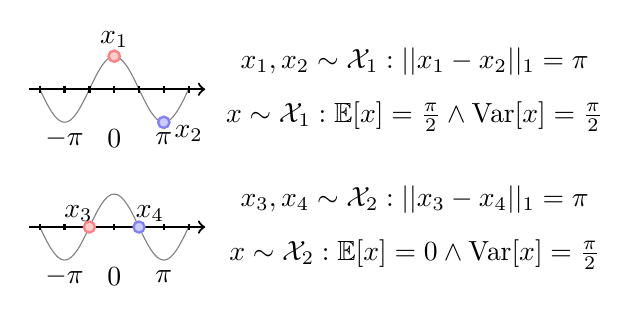
\begin{tikzpicture}
        [scale=0.7,
        inner sep=0.5mm,
        pd/.style={circle,draw=red!50,fill=red!20,thick},
        hc/.style={circle,draw=blue!50,fill=blue!20,thick}]
        
        \node (sinusoid1) at (0,0) {};
        
        \draw[black, thick, ->] ($(sinusoid1)+(-2,0.3)$) -- ($(sinusoid1)+(1.2,0.3)$);%xaxis
        \draw[thin, black!50] ($(sinusoid1)+(0.9,0.3)$) sin ($(sinusoid1)+(0.45,-0.3)$);
        \draw[thin, black!50] ($(sinusoid1)+(0.45,-0.3)$) cos ($(sinusoid1)+(0.,0.3)$);
        \draw[thin, black!50] ($(sinusoid1)+(0.,0.3)$) sin ($(sinusoid1)+(-0.45,0.9)$);
        \draw[thin, black!50] ($(sinusoid1)+(-0.45,0.9)$) cos ($(sinusoid1)+(-0.9,0.3)$);
        \draw[thin, black!50] ($(sinusoid1)+(-0.9,0.3)$) sin ($(sinusoid1)+(-1.35,-0.3)$);
        \draw[thin, black!50] ($(sinusoid1)+(-1.35,-0.3)$) cos ($(sinusoid1)+(-1.8,0.3)$);
        
        
        \draw[black, thick] ($(sinusoid1)+(-1.8,0.36)$) -- ($(sinusoid1)+(-1.8,0.24)$);
        \draw[black, thick] ($(sinusoid1)+(-1.35,0.36)$) -- ($(sinusoid1)+(-1.35,0.24)$);
        \draw[black, thick] ($(sinusoid1)+(-0.9,0.36)$) -- ($(sinusoid1)+(-0.9,0.24)$);
        \draw[black, thick] ($(sinusoid1)+(-0.45,0.36)$) -- ($(sinusoid1)+(-0.45,0.24)$);
        \draw[black, thick] ($(sinusoid1)+(0.,0.36)$) -- ($(sinusoid1)+(0.,0.24)$);
        \draw[black, thick] ($(sinusoid1)+(0.45,0.36)$) -- ($(sinusoid1)+(0.45,0.24)$);
        \draw[black, thick] ($(sinusoid1)+(0.9,0.36)$) -- ($(sinusoid1)+(0.9,0.24)$);
        
        \node at ($(sinusoid1)+(-1.35,-0.6)$) {$-\pi$};
        \node at ($(sinusoid1)+(-0.45,-0.6)$) {$0$};
        \node at ($(sinusoid1)+(0.45,-0.6)$) {$\pi$};
        
        \node (ind1) at ($(sinusoid1)+(-0.45,0.9)$) [pd] {};
        \node (ind1) at ($(sinusoid1)+(0.45,-0.3)$) [hc] {};
        
        \node (ind1) at ($(sinusoid1)+(-0.45,0.9)$) [pd] {};
        \node (ind1) at ($(sinusoid1)+(0.45,-0.3)$) [hc] {};
        
        
        \node (sinusoid2) at ($(sinusoid1)+(0,-2.5)$) {};
        
        \draw[black, thick, ->] ($(sinusoid2)+(-2,0.3)$) -- ($(sinusoid2)+(1.2,0.3)$);%xaxis
        \draw[thin, black!50] ($(sinusoid2)+(0.9,0.3)$) sin ($(sinusoid2)+(0.45,-0.3)$);
        \draw[thin, black!50] ($(sinusoid2)+(0.45,-0.3)$) cos ($(sinusoid2)+(0.,0.3)$);
        \draw[thin, black!50] ($(sinusoid2)+(0.,0.3)$) sin ($(sinusoid2)+(-0.45,0.9)$);
        \draw[thin, black!50] ($(sinusoid2)+(-0.45,0.9)$) cos ($(sinusoid2)+(-0.9,0.3)$);
        \draw[thin, black!50] ($(sinusoid2)+(-0.9,0.3)$) sin ($(sinusoid2)+(-1.35,-0.3)$);
        \draw[thin, black!50] ($(sinusoid2)+(-1.35,-0.3)$) cos ($(sinusoid2)+(-1.8,0.3)$);
        
        
        \draw[black, thick] ($(sinusoid2)+(-1.8,0.36)$) -- ($(sinusoid2)+(-1.8,0.24)$);
        \draw[black, thick] ($(sinusoid2)+(-1.35,0.36)$) -- ($(sinusoid2)+(-1.35,0.24)$);
        \draw[black, thick] ($(sinusoid2)+(-0.9,0.36)$) -- ($(sinusoid2)+(-0.9,0.24)$);
        \draw[black, thick] ($(sinusoid2)+(-0.45,0.36)$) -- ($(sinusoid2)+(-0.45,0.24)$);
        \draw[black, thick] ($(sinusoid2)+(0.,0.36)$) -- ($(sinusoid2)+(0.,0.24)$);
        \draw[black, thick] ($(sinusoid2)+(0.45,0.36)$) -- ($(sinusoid2)+(0.45,0.24)$);
        \draw[black, thick] ($(sinusoid2)+(0.9,0.36)$) -- ($(sinusoid2)+(0.9,0.24)$);
        
        \node at ($(sinusoid2)+(-1.35,-0.6)$) {$-\pi$};
        \node at ($(sinusoid2)+(-0.45,-0.6)$) {$0$};
        \node at ($(sinusoid2)+(0.45,-0.6)$) {$\pi$};
        
        \node (ind1) at ($(sinusoid2)+(-0.9,0.3)$) [pd] {};
        \node (ind1) at ($(sinusoid2)+(0.,0.3)$) [hc] {};
        
        
        \node at ($(sinusoid1)+(-0.45,1.2)$) {$x_1$};
        \node at ($(sinusoid1)+(0.9,-0.5)$) {$x_2$};
        
        \node at ($(sinusoid2)+(-1.1,0.55)$) {$x_3$};
        \node at ($(sinusoid2)+(0.2,0.55)$) {$x_4$};
        
        \node (distance1) at ($(sinusoid1)+(5,0.8)$) {$x_1, x_2 \sim \mathcal{X}_1: ||x_1-x_2||_1=\pi$};
        \node at ($(distance1)+(0,-1)$) {$x \sim \mathcal{X}_1: \mathbb{E}[x] = \frac{\pi}{2} \wedge \mbox{Var}[x]=\frac{\pi}{2}$};
        
        \node (distance2) at ($(sinusoid2)+(5,0.8)$) {$x_3, x_4 \sim \mathcal{X}_2: ||x_3-x_4||_1=\pi$};
        \node at ($(distance2)+(0,-1)$) {$x \sim \mathcal{X}_2: \mathbb{E}[x] = 0 \wedge \mbox{Var}[x]=\frac{\pi}{2}$};
    \end{tikzpicture}
\end{document}
